
\documentclass[a4paper,twoside,openright,12pt,Slovene]{book}
\usepackage[pdftex]{UNI-LJ-FE-Diploma} % stil zaključnega dela UL FE
\usepackage[utf8]{inputenc} % predloga uporablja standardno kodiranje Unicode UTF-8, ki podpira šumnike
\usepackage[greek,english,Slovene]{babel} % seznam uporabljenih jezikov (zadnji na seznamu je primarni)


\usepackage{filecontents}
\begin{filecontents*}{\jobname.xmpdata}
    \Title{Simulator elektrostatične raztelektritve} % Mora biti enak kot je v prijavi teme!
    \Author{Vid Oblak} % Mora biti enak kot na naslovnici!
\end{filecontents*}
\usepackage[a-1b]{pdfx}
%%%%%%%%%%%%%%%%%%%%%%%%%%%%%%%%%%%%%%%%%%%%%%%%%%%%%%%%%%%%%%%%%%%%%%%%%%%%%%%%%%%%%%%%%%%%%%%%%%%%%%%%%%%%%%%%%%%%%%%%


% Kompakten pregled LaTeX ukazov je dostopen na https://en.wikibooks.org/wiki/Category:Book:LaTeX
% Navodila posameznih uporabljenih paketov so dostopna na https://www.ctan.org

% Dodatni simboli
\usepackage{textcomp}                               % dodatni simboli (kot npr. €)
\usepackage{gensymb}                                % dodatni simboli \de­gree, \cel­sius, \pert­hou­sand, \mi­cro, \ohm
\newcommand{\uppi}{\textrm{\greektext p\latintext}} % velika grška črka P z \uppi, alternativa simbolu \Pi

% Osnovno oblikovanje
\hypersetup{unicode,hidelinks,breaklinks,hyperindex} % dodatne možnosti hiperpovezav
\usepackage[normalem]{ulem}                          % podčrtavanje in prečrtavanje teksta
\usepackage{float}                                   % dodatne možnosti oblikovanja objektov
\usepackage{enumitem}                                % dodatne možnosti oblikovanja seznamov

% Dodatno oblikovanje
%\zamaknirobsodihstrani{0mm} % dodatna prilagoditev levega roba sodih strani za dvostranski tisk
%\usepackage{dcolumn}        % poravnava po decimalnih mestih v tabelah
%\usepackage{longtable}      % večstranske tabele
%\usepackage{caption}        % dodatne možnosti označevanja objektov
%\usepackage{rotating}       % vretenje objektov, strani, ipd.

\usepackage{siunitx} %uporaba SI simbolov

% Matematična orodja
\usepackage{mathtools} % http://mirrors.ctan.org/macros/LaTeX/contrib/mathtools/mathtools.pdf
\usepackage{bm}        % ukaz za odebeljeni tisk \bm v matematičnih okoljih
%\usepackage{cancel}   % ukaz za prečrtavanje \cancel v matematičnih okoljih

% Grafična orodja
\usepackage{graphicx}                 % vključevanje bitnih slik z ukazom \includegraphics
\usepackage{grffile}                  % podpora presledkom pri ukazu \includegraphics
%\usepackage{tikz}                    % paket TikZ za risanje (npr. blokovnih shem, diagramov poteka, itd.)
%\usetikzlibrary{calc,shapes,arrows}  % dodatne možnosti paketa TikZ
%\usepackage{tikzscale}               % skaliranje risb
\usepackage[smartlabels, european, americaninductors]{circuitikz} % risanje shem vezij
%\usepackage{pgfplots}                % paket PGFPlots za risanje grafov, tudi iz CSV in podobnih datotek
%\usepgfplotslibrary{polar,external}  % dodatne možnosti paketa PGFPlots
%\usepackage{tikz-3dplot}             % 3D risanje
% Primeri: http://texample.net , http://pgfplots.net/tikz/examples , http://pgfplots.sourceforge.net/gallery.html

% Vključevanje datotek
\usepackage{pdfpages} % vključevanje PDF datotek z ukazom \includegraphics
\usepackage{epstopdf} % vključevanje EPS datotek z ukazom \includegraphics
\usepackage{listings} % orodja za izpisovanje programske kode
\lstset{              % nastavitve orodja za izpisovanje programske kode
    basicstyle=\ttfamily\footnotesize,
    breaklines=true,
    numbers=left,
    numberstyle=\scriptsize,
    keywordstyle=\color{blue},
    commentstyle=\color{unilj},
    stringstyle=\color{olive},
}
%%%%%%%%%%%%%%%%%%%%%%%%%%%%%%%%%%%%%%%%%%%%%%%%%%%%%%%%%%%%%%%%%%%%%%%%%%%%%%%%%%%%%%%%%%%%%%%%%%%%%%%%%%%%%%%%%%%%%%%%

% DEKLARACIJE %%%%%%%%%%%%%%%%%%%%%%%%%%%%%%%%%%%%%%%%%%%%%%%%%%%%%%%%%%%%%%%%%%%%%%%%%%%%%%%%%%%%%%%%%%%%%%%%%%%%%%%%%%
\naslov{Simulator elektrostatične razelektritve} % Mora biti enak kot je v prijavi teme!
\avtor{Vid Oblak} % Mora se ujemati s \Title pri metapodatkih PDF/A!
\mentor{Izr. Prof. Dr. Peter Zajec}
%\somentor{Naziv, ime in priimek somentorja}
\date{Ljubljana, \the\year}
\univerza{Univerza v Ljubljani}
\definecolor{unilj}{cmyk}{0.00, 0.94, 0.94, 0.06} % barva Univerze v Ljubljani

\delo{Poročilo o delu\\~\\Visokošolski strokovni študijski program\\prve stopnje Aplikativna elektrotehnika}
\fakulteta{Fakulteta za elektrotehniko}

% DOKUMENT %%%%%%%%%%%%%%%%%%%%%%%%%%%%%%%%%%%%%%%%%%%%%%%%%%%%%%%%%%%%%%%%%%%%%%%%%%%%%%%%%%%%%%%%%%%%%%%%%%%%%%%%%%%%%
\begin{document}

\frontmatter

\selectlanguage{slovene}

%******************************* NASLOVNICA ************************************
\maketitle

%******************************* ZAHVALA ***************************************
\zahvala
Zahvaljujem se mentorju dr. Petru Zajcu in mentorju v podjetju Blažu Prahu, katera sta mi pomagala z nasveti, izračuni in realizacijo projekta. Zahvaljujem se tudi sodelavcu Janu Pogačarju, ki je vskočil na pomoč pri uporabi Python in LaTeX. Prav tako se zahvaljujem vsem ostalim sodelavcem in prijateljem, kateri so tudi v najmanjši meri pomagali pri razvoju ali realizaciji projekta.


%******************************* POVZETEK IN KLJUČNE BESEDE ********************
\povzetek
V tem zaključnem poročilu je opisan razvoj simulatorja elektrostatične razelektritve za integrirana vezja in problemov, ki sem jih imel pri razvoju. 

Simulator je sestavljen iz treh glavnih modulov in sicer kontrolne ploščice, nastavljivega visokonapetostnega napajalnika in visokonapetostnega stikala.
Zaradi trenutne gospodarske situacije smo se tekom razvoja projekta odločili, da bomo pri razvoju simulatorja poskušali čimbolj zmanjšati stroške. Ta odločitev je pomenila dodaten razvoj in izdelavo nastavljivega visokonapetostnega napajalnika in visokonapetostnega stikala, namesto nakupa le teh. 
Vsi moduli projekta so bili načrtovani z modularnostjo v mislih, da v primeru kasnejše nadgradnje ali zamenjave, le-ta poteka čim bolj nemoteno. 

Tekom projekta sem prišel do spoznanja, da bi izdelava simulatorja, ki bi ustrezal vsem standardom, zahtevala precej več časa in bistveno večji proračun.

\kljucnebesede
ESD, Elektrostatika, Simulator elektrostatične razelektritve, mikroelektronika

\selectlanguage{english}

%******************************* ABSTRACT AND KEYWORDS *************************

\abstract
In this final report is description of development of ESD simulator for microelectronics and problems experienced during development. 

Simulator has been composed of three main modules: main control board, adjustable high-voltage power supply and high-voltage switch. Due to current economy situation we have decided to focus on low cost simulator production. This meant development and manufacturing of our own adjustable high-voltage power supply and high-voltage switch, instead of purchasing. All modules of the simulator were designed to be modular and swappable, that way upgrades or replacements can be made without major disruption. 

During development I have come to conclusion that ESD simulator which would compy with requirements can not be made in specified time frame and defined budget.

\keywords
ESD, Electrostatic, ESD Simulator, microelectronics

\selectlanguage{slovene}

%******************************* KAZALO ****************************************
\tableofcontents

%******************************* SEZNAM SLIK, SEZNAM TABEL *********************
\seznamslik
\seznamtabel

%******************************* SEZNAM SIMBOLOV *******************************
\seznamsimbolov
V pričujočem zaključnem delu, so uporabljene naslednje veličine in simboli:

\begin{center}
    \begin{tabular}{*{4}{l}} \hline
        \multicolumn{2}{c}{\bf{Veličina / oznaka}}           & \multicolumn{2}{c}{\bf{Enota}} \\ \hline
        Ime                & Simbol                          & Ime      & Simbol              \\ \hline
        čas                & $t$                             & sekunda  & s                   \\
        frekvenca          & $f$                             & Hertz    & Hz                  \\
        napetost           & $U$                             & Volt     & V                  \\
        tok                & $I$                             & Amper    & A                   \\
        upornost           & $R$                             & Ohm      & $\Omega$            \\ \hline

    \end{tabular}
\end{center} 

\noindent
Natančnejši pomen simbolov ter njihovih indeksov je razviden iz ustreznih slik ali pa je pojasnjen v spremljajočem besedilu, kjer je simbol uporabljen.

\mainmatter

%******************************* UVOD ******************************************
\chapter{Uvod} \label{uvod}

Praktično usposabljanje sem opravljal v podjetju Renishaw d.o.o., ki je hčerinsko podjetje Britanskega inžinerskega podjetja Renishaw p.l.c.  Podjetje razvija integrirana vezja za specifično uporabo (ASIC). 

Inžinerji v podjetju so razdeljeni na tri skupine:
\begin{itemize}
	\item Načrtovalci: načrtujejo posamezne sklope integriranega vezja in karakterizirajo vezje s pomočjo simulacij.
	\item Oblikovalci sestavnice mask: postavijo posamezne komponente na površino integriranega vezja (podobno kot risanje tiskanih vezij).
	\item Testni inženirji: karakterizirajo narejena integrirana vezja, načrtujejo testna vezja in skrbijo za testiranje vezij za proizvodnjo.
\end{itemize}
Sam sem izvajal praktično usposabljanje v skupini testnih inženirjev. Tej skupini sem se sam pridružil že pred tremi leti. V tem času sem dobro spoznal vse postopke, zato sem lahko takoj začel z izvajanjem zasnove in izdelave projekta. Zadana mi je bila naloga zasnove in izdelave simulatorja elektrostatične razelektritve, ki se uporablja pri verifikaciji integriranih vezij. Zahteve so bile naslednje:
\begin{itemize}
	\item Maksimalna izhodna napetost vsaj \SI{15}{\kilo\volt} DC,
	\item Nastavljanje izhodne napetosti med \SI{250}{\volt} in \SI{15}{\kilo\volt},
	\item Natančnost izhodne napetosti vsaj 3\%,
	\item Zagotavljanje skladnosti z vsemi ustreznimi zahtevami na nivoju EU (pridobitev oznake CE).
\end{itemize}


\begin{figure}[H]
	\centering
    \begin{circuitikz}
        \draw (0,0)
       to[V, v=$V$] (0,3)
       to[R=1M] (2,3)
       to[short] (2.685,3)
       to[short] (2.685,2.5);
       
       \draw (3,2)
       node[spdt, rotate=90] {};
       
       \draw (0,0)
       to[short] (3,0)
       to[C=100pF] (3,1.5);
       
       \draw (3,0)
       to[short] (5,0)
       to[short, -d] (5,0.5);
       
       \draw (3.315,2.5)
       to[short] (3.315,3)
       to[R=1500Ohm] (5,3)
       to[short, -d] (5,2.5);
       
       
    \end{circuitikz}
          \caption{\label{ESDTesterShemaOsnovna} Osnovna shema ESD simulatorja.}
    \end{figure}

Za potrebe testiranja integriranih vezij so v podjetju potrebovali simulator elektrostatične razelektritve. Na začetku snovanja so bile zastavljene specifikacije maksimalne napetosti \SI{15}{\kilo\volt} in uporaba že narejenih modulov za nastavljivi visokonapetostni napajalnik ter visokonapetostno stikalo. Tekom projekta se je to spremenilo in prišlo do odločitve o lastnem načrtovanju nastavljivega visokonapetostnega napajalnika. Pri tem modulu sem moral premostit kar nekaj tehničnih ovir. Največji sta bili zagotovitev skladnosti z vsemi ustreznimi zahtevami na nivoju EU ter zagotavljanje \SI{15}{\kilo\volt} izolacije med primarno in sekundarno stranjo.   

Princip delovanja simulatorja elektrostatične razelektritve je dokaj enostaven. Nastavljivi visokonapetostni vir polni kondenzator, katerega se nato preko upora prazni skozi testiranec.    
Prvotni načrt je bil lastno navijanje primernega visokonapetostnega transformatorja. Po kar nekaj meritvah in izračunih se je to pokazalo za neizvedljivo, saj nismo uspeli zagotoviti želene napetosti in izolacije. Rezervni načrt je bil razdreti televizor s katodno cevjo in od tam vzeti transformator. Vendar pa smo se temu želeli izogniti zaradi nedostopnosti takih televizorjev, ki jih bo z letu vedno manj. Motilo me je pa tudi razlikovanje transformatorjev tako v podnožju kot tudi v karakteristikah, vgrajene diode v sekundarnem navitju še dodatno otežijo karakterizacijo transformatorja. 
Težave je povzročala tudi regulacija napetosti zaradi zagotavljanja potrebne galvanske izolacije. S pomočjo simulacij sem preizkusil kateri tipi napetostnih krmilnikov bi ustrezali. Tako so bili izločeni vsi neizolirani krmilniki. Krmilnik s povratno vezavo preko optičnega spojnika namreč ni zmožen pokrivati celotne izhodne napetosti od \SI{250}{\volt} do \SI{15}{\kilo\volt} zaradi nelinearnosti, krmilnik s povratno vezavo preko pomožnega navitja pa se je v simulacijah zdel obetavno, vendar se je na koncu izkazal za neprimernega. Primeren je bil samo regulator, ki ima povratno vezavo preko primarnega navitja in sicer s merjenjem zrcaljene napetosti z sekundarnega navitja na primarno. Po obsežnejših meritvah pa se je tudi ta izkazal za neprimernega. Na koncu je bilo potrebno izdelati regulator z mikrokrmilnikom, kateri prejema povratno vezavo preko galvansko ločenega analogno-digitalnega pretvornika.
Po standardih MIL-STD-883K ~\cite{MIL-STD-883K} in JS-001-2007 ~\cite{JS-001-2017} mora biti visokonapetostno stikalo, katero prazni kondenzator skozi testiranec t.i. ''bounce-less'', se pravi ko sklene kontakt ga mora zadržati, namesto, da ga na kratko večkrat razklene in sklene. Standarda pa tudi predpisujeta obliko signala toka skozi testiranec, zato razbremenilno vezje t.i. ''snubber'' čez kontakte stikala ni primerna rešitev. Za nižje napetosti obstajajo releji, kateri vsebujejo živo srebro, čigar naloga je zadržati kontakt, ko se kontakta odbijeta. Vendar cena takšnega releja za \SI{15}{\kilo\volt} znaša okoli \texteuro2000.
Kompromis je bil izdelava lastnega stikala, ki bo ustrezalo zahtevam.





%******************************* POGLAVJA **************************************
\chapter{Simulator elektrostatične razelektritve} \label{ESDSIM}

	\section{Praktično usposabljanje}
	Načrtovalski del projekta sem izvajal na svojem računalniškem delovnem mestu, kjer sem uporabljal:
	\begin{itemize}
		\item Altium Designer: risanje električnih shem in načrtovanje tiskanih vezij.
		\item Visio: risanje blok diagramov in konceptnih shem.
		\item LTSpice: simulacija analognih vezij.
		\item STM32Cube: programiranje mikrokrmilnikov ARM STM32.
		\item Python: komunikacija med mikrokrmilnikom in računalnikom.
	\end{itemize}
	Na svoji delovni mizi sem imel nameščeno antistatično podlogo, toda to delovno mesto ni bilo primerno za izvajanje meritev (potencialno za izvajanje hitrih meritev) s katerimi je bil potrjen koncept.
	Za obsežnejše meritve sem imel na voljo merilno mesto, kjer je bilo na voljo več merilnih inštrumentov. 
	
	Pri svojem delu sem največ uporabljal:
	\begin{itemize}
		\item Rigol DS1054Z: digitalni osciloskop.
		\item Acute ADP2100 : visokonapetostna diferencialna sonda.
		\item Rigol DP832: 3 kanalni laboratorijski napajalnik.
		\item PeackTech 3450: multimeter z vgrajeno termalno kamero.
	\end{itemize}
	Pred delom z visoko napetostjo sem moral opraviti interni tečaj varstva pri delu z visoko napetostjo. Po posvetu z mentorjem sva sklenila razdeliti nalogo na posamezne module. Za vsak modul sem naprej pripravil blokovno shemo ter opis možnih rešitev, po pregledu le teh je sledilo nadaljnje simuliranje v LTSpice in po potrditvi rezultatov še načrtovanje v Altium Designer.
	
	\section{Zasnova simulatorja elektrostatične razelektritve}
	Poleg že omenjenih specifikacij je veljalo tudi, da mora simulator ustrezati standardoma MIL-STD-883K in JS-001-2007. Osnovna shema simulatorja je sledeča:
	\begin{figure}[h]
	\centering
    \begin{circuitikz}
        \draw (0,0)
       to[V, v=$V$] (0,3)
       to[R=1M] (2,3)
       to[short] (2.685,3)
       to[short] (2.685,2.5);
       
       \draw (3,2)
       node[spdt, rotate=90] {};
       
       \draw (0,0)
       to[short] (3,0)
       to[C=100pF] (3,1.5);
       
       \draw (3,0)
       to[short] (5,0)
       to[short, -d] (5,0.5);
       
       \draw (3.315,2.5)
       to[short] (3.315,3)
       to[R=1500Ohm] (5,3)
       to[short, -d] (5,2.5);
    \end{circuitikz}
          \caption{\label{ESDTesterShemaOsnovna} Osnovna shema ESD simulatorja.}
    \end{figure}
    
	Sestavljajo ga nastavljivi visokonapetostni izvir, polnilni upor, praznilni kondenzator, praznilni upor ter ne-preskakovalno (t.i. bounce-less) stikalo. Praznilni kondenzator se preko polnilnega upora napolni na želeno napetost, preko praznilnega upora pa se sprazni skozi testiranec. Izhodni tok mora ustrezati limitam, katere so podane v standardih: dvižni čas mora biti manjši kot \SI{10}{\nano\second} ter nominalni čas praznjenja kondenzatorja skozi kratek stik mora biti \SI{150}{\nano\second}, z maksimalnim odstopanjem \SI{\pm 20}{\nano\second}. Slednja zahteva pomeni, da smemo s stikalom, povezovalnimi žicami in konektorji smemo dodati maksimalno \SI{20}{\pico\farad} parazitne kapacitivnosti, ker bo sicer izpraznitve skozi kratek stik odstopal od zahtevanega. Pri načrtovanju visokonapetostnega izvira je prav tako potrebno biti previden, saj mora le-ta zagotavljati \SI{15}{\kilo\volt} izolacije med primarno in sekundarno stranjo.
%diplomska - slika grafa iz standarda

	\subsection{Moduli simulatorja}
	Simulator je sestavljen iz 4 modulov, od katerih vsak opravlja posebno nalogo.
	\begin{figure}[h]
    \centering
    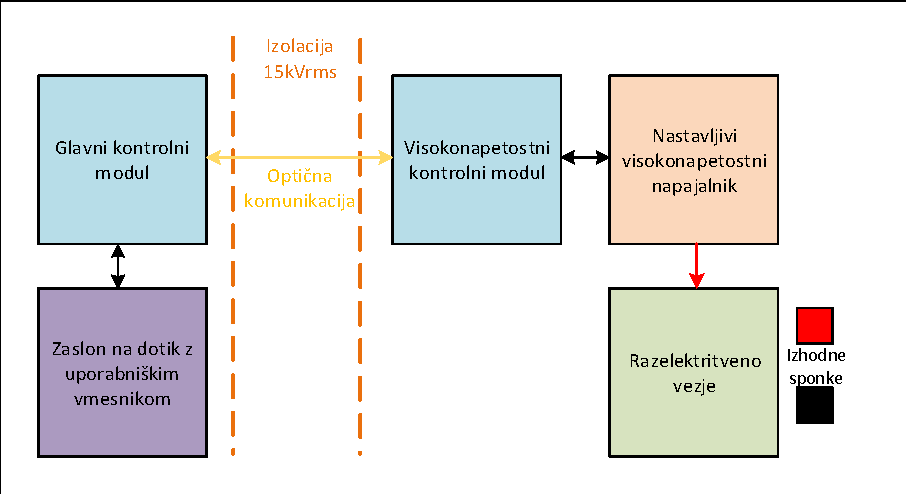
\includegraphics[width=1\columnwidth]{Sheme/Osnovna blok shema poenostavljena.pdf}
    \caption{\label{BlokDiagramShema} Shema blok diagrama.}
	\end{figure}
	
	\begin{itemize}
		\item Glavni kontrolni modul: krmili visokonapetostni modul, prejema uporabnikove ukaze preko zaslona na dotik, pošilja podatke po LAN ali USB.
		\item Visokonapetostni kontrolni modul: krmili nastavljivi visokonapetostni napajalnik in razelektritveno vezje glede na ukaze glavnega kontrolnega modula, varnostno odklaplja napajanje nastavljivega napajalnika, ko le-ta ni v uporabi.
		\item Nastavljivi visokonapetostni napajalnik: glede na zahteve regulira enosmerno napetost od \SI{250}{\volt} do \SI{15}{\kilo\volt}.
		\item Razelektritveno vezje: izprazni naboj iz praznilnega kondenzatorja preko testiranca.
	\end{itemize}

	\subsection{Nastavljivi visokonapetostni napajalnik}
	Začel sem z nastavljivim visokonapetostnim napajalnikom, saj sem pričakoval, da se bom z njim največ zamudil in na koncu so se moja predvidevanja izkazala za pravilna. Z visokimi napetostmi nisem imel izkušenj, imel pa sem izkušnje z Cockcroft-Walton-ovim množilnikom napetosti. Zamislil sem si stikalni napajalnik, ki bi pretvarjal \SI{24}{\volt} v \SI{250}{\volt}, za njim pa 60 stopenj množilnika. Regulaciji napetosti na transformatorju bi sledila tudi izhodna napetost množilnika. Po simulacijah sem hitro ugotovil, da to ne bo delovalo po pričakovanjih, saj so kapacitivne izgube previsoke. Prvotna ideja je bila dodati samo nekaj stopenj, vendar sem hitro ugotovil, da kljub dodatku 60 stopenj ne bom mogel doseči \SI{15}{\kilo\volt} iz \SI{250}{\volt}. V članku avtorja Hanington, G~\cite{ParallelHighVoltageMultipliers} je opisan podoben problem. Za napajanje nevtronskih generatorjev so potrebovali \SI{100}{\kilo\volt} DC, njihova rešitev za kapacitivne izgube je uporaba paralelnega napetostnega množilnika. 
	
	Po računih in simulacijah je rešitev izgledala obetavno. Navdušen nad rezultati sem se lotil risanja sheme in tiskanega vezja v Altium Designerju, kjer pa se je lahko hitro opazila kritična napaka. Za povratno zanko regulacije je bil uporabljen analogno-digitalni pretvornik s primerno dimenzioniranim pred-uporom in s tem je bila prekinjena galvanska izolacija med primarnim in sekundarnim navitjem. Na srečo je bila moja napaka diagnosticirana, preden smo dali tiskano vezje v izdelavo. Po pogovoru s sodelavci sem ugotovil, da bo transformator verjetno najboljša opcija za dvigovanje napetosti. Po izvedbi povpraševanj pri večjih ponudnikih elektronskih komponent sem prišel do zaključka, da primernega transformatorja ne bo možno kupiti, pač pa ga bo potrebno narediti. V preteklosti sem že navijal omrežne transformatorje, z načrtovanjem transformatorjev za navzgor (t.i. ''flyback'') pa nisem imel še nobenih izkušenj. Za začetek sem uporabil jedra RM10 iz materiala N87, ki so bila na zalogi. Predhodno sem izračunal, koliko ovojev potrebujem na primarni strani, preden preide jedro v nasičenje pri \SI{3}{\ampere}. Navil sem transformator z razmerjem 1:10 in enega z razmerjem 1:20.
%TODO Meritve
Za meritve sem potreboval še napetostni delilnik za visokonapetostno sondo, saj je le ta narejena samo za \SI{1.8}{\kilo\volt}. Po specifikacijah ima vhodno upornost \SI{2}{\mega\ohm}, kar pomeni da z pred-uporom \SI{18}{\mega\ohm} dosežemo razmerje 1:10 in posledično maksimalno napetost \SI{18}{\kilo\volt}. Pri tem nisem dodal kapacitivne kompenzacije, zato je sonda bolj uporabna za indikacijo, kot pa za meritve. Tuljavo sem krmilil s pomočjo MOSFETa in namenskega krmilnika vrat UCC27517~\cite{TI:UCC27517} proizvajalca Texas Instruments. 
Le-ta zaradi izredno kratkega časa vzpona in padca, omogoča opravljanje meritve tudi pri višjih frekvencah. Maksimalni izhodni tok \SI{4}{\ampere} omogoča hitro odpiranje/zapiranje MOSFETov z višjim \(U_{DS}\). S signalnim generatorjem se lahko natančno kontrolira krmilnik. Meritve so opravljene pri napetostih \SI{5}{\volt}, \SI{10}{\volt} in \SI{15}{\volt} ter spremenjenemu delovnem ciklu od \SI{0.1}{\percent} do \SI{10}{\percent} delovnega cikla. Ugotovil sem, da se pri delovnih ciklih nad \SI{10}{\percent} izhodna napetost ne spreminja več, oziroma transformator preide v nasičenje in posledično se zelo segreje. Omejitev toka je bila nastavljena \SI{3}{\ampere}, pa ni bilo tako pomembno zaradi paralelno vezanega elektrolitskega kondezatorja s kapacitivnostjo \SI{4700}{\micro\farad} in izhodnih sponk. Meritve so pokazale, da napetost \(U_{pp}\) lahko brez problema doseže zahtevanih \SI{15}{\kilo\volt}, vendar prihaja do preboja napetosti med navitji transformatorja. Odločil sem se narediti še dodatne meritve s tremi različnimi jedri. Pri iskanju jedra, sem si pomagal s skripto napisano v Matlabu, kateri mi glede na \(A_L\) in \(l_e\) parametre izračuna potrebno razmerje navojev ter maksimalni magnetilni tok. Izbrana so bila naslednja jedra: EFD 30/15/9, PM 50/39 in E 70/33/32 z \SI{1.5}{\milli\meter} režo. Večja transformatorja sta bila precej obetavna, saj bi na tuljavniku lažje zagotavljali primerno izolacijo. Visoka \(A_L\) vrednost pomeni manjše število ovojev. Iz radovednosti sem pomeril tudi dva transformatorja navzgor, katera sem sta prispela kot vzorca proizvajalca CoilCraft in sicer GA3459~\cite{Coilcraft:GA3459} in GA3460, sta pa namenjena za \SI{500}{\volt}. Po meritvah se je izkazalo, da transformatorja z velikim jedrom delujeta pod pričakovanji, transformatorja proizvajalca CoilCraft pa delujeta izredno dobro in skoraj dosegata želene napetosti, najbolje pa se je izkazal mali transformator z EFD jedrom. 
 
\begin{table}[h!]
\centering
\begin{tabular}{||c|c|c|c|c|c|c||}
\hline
Ime & \(L_{pri}\) & \(L_{sec}\) & Razmerje & \(U_{pp MAX}\) & Jedro & Reža \\ [0.5ex]
\hline\hline
GA3460 & \SI{2.6}{\micro\henry} & \SI{253}{\micro\henry} & 1:10 & \SI{3.9}{\kilo\volt} & EFD 25/13/9 & \SI{0.5}{\milli\meter} \\
\hline
GA3459 & \SI{5}{\micro\henry} & \SI{505}{\micro\henry} & 1:10 & \SI{13.8}{\kilo\volt} & EFD 25/13/9 & \SI{0.5}{\milli\meter} \\
\hline
Mali z EFD & \SI{76}{\micro\henry} & \SI{13.21}{\milli\henry} & 1:13 & \SI{7.84}{\kilo\volt} & EFD 30/15/9 & \SI{0}{\milli\meter} \\
\hline
\end{tabular}

\caption{Ožji izbor transformatorjev}

\end{table}

Z rezultati meritev še nisem bil popolnoma zadovoljen, vendar sem se vseeno odločil, vendar sem se odločil najprej ugotoviti način regulacije izhodne napetosti in si kasneje po potrebi prilagoditi parametre transformatorja. 

	\subsubsection{Regulacija napetosti} \label{RegulacijaNapetosti}
	Prvotno sem si želel skrajšati čas načrtovanja in vzeti že narejeni regulator in po potrebi prilagoditi vezje okoli njega - vezje povratne zanke. Glede na obstoj številnih krmilnikov namenjenih za navzgor topologijo, sem med njimi začel iskanje najprimernejšega začel iskanje primernih. V ožji izbor sem uvrstil:
	
\begin{table}[h!]
\centering
\begin{tabular}{||c | c |c||}
\hline
Ime & Proizvajalec & Način povratne zanke \\[0.5ex]
\hline\hline
LM5155 & Texas Instruments & Optoizolator \\
UCC28740-Q1 & Texas Instruments & Optoizolator \\
LT3748 & Linear Technology & Zaznavanje na primarnem navitju \\
LT3757 & Linear Technology & Napetostni delilnik na izhodu \\
LT8304 & Linear Technology & Zaznavanje na primarnem navitju \\ [1ex]

\hline
\end{tabular}
\caption{Ožji izbor regulatorjev}
\end{table}

	\subsubsection{LM5155} \label{LM5155}
Krmilnik LT5155~\cite{TI:LT5155} ima avtomatsko regulacijo frekvence v območju od \SI{170}{\hertz} do \SI{100}{\kilo\hertz}. Povratna vezava je izolirana preko optičnega spojnika, ki je prožen na izhodni strani preko napetostnega delilnika in Zenner diode. S spreminjanjem vrednosti upora povratne vezave se spreminja točka, pri kateri se proži optični spojnik. Kljub ponovnim izračunom in dvojnim preverjanjem sheme ta krmilnik ni deloval v simulacijskem okolju, dolg čas dobave pa je onemogočil prototipni test.


	\subsubsection{UCC28740-Q1} \label{UCC28740-Q1}
UCC28740-Q1~\cite{TI:UCC28740} deluje po enakem principu kot že omenjeni LM5155. Ta krmilnik je namenjen delovanju usmerjeni omrežni napetosti, saj od tam dobi podatek o referenčni frekvenci. Takšen krmilnik ni uporaben, saj se nastavljivi visokonapetostni regulator napaja iz \SI{24}{\volt} DC. 



	\subsubsection{LT3748} \label{LT3748}
Krmilnik elegantno rešuje moj problem, saj ne potrebuje dodatne povratne vezave, informacijo o izhodni napetosti namreč dobi preko zrcaljene napetosti na primarnem navitju. Ko se izključi N Kanalni MOSFET, napetost na ponoru zraste nad vhodno napetost, katera je enaka \(V_{FLBK} = (V_{OUT} + V_F + I_{SEC} * ESR) * N_{PS}) \). Pri tem je \(V_{FLBK}\) zrcaljena napetost, \(V_F\) pragovna napetost izhodne diode, \(I_{SEC}\) tok na sekundarnem navitju, \(ESR\) skupna impedanca vezja na sekundarni strani in \(N_{PS}\) razmerje navojev med primarnim in sekundarnim navitjem. Ta napetost steče proti masi preko upora za nastavitev napetosti \(R_{FB}\) in interno zaporedno vezanim \(R_{REF}\), točka med uporoma je vezana na invertirajoči vhod ojačevalnika napake z referenco \(V_{BG}\) \SI{1.223}{\volt} \cite{analog:LT3748}. Izhodna napetost je enaka \(V_{OUT} = V_{BG}(R_{FB} / R_{REF})(1 / N_{PS}) - V_F - I_{SEC} (ESR)\), kjer lahko pri naših napetostih zanemarimo \(V_F\) in \(I_SEC (ESR)\), upoštevati pa moramo tudi zahteve za minimalno induktivnost primarnega navitja:
\[L_{PRI} \geq \frac{(V_{OUT}+V_{F(DIODE)}) * R_{SENSE} * t_{Settle(MIN)} * N_{PS}}{V_{Sense(MIN}}\]
\[V_{SENSE(MIN)}=\SI{15}{\milli\volt}\]
\[t_{SETTLE(MIN)}=\SI{400}{\nano\second}\]
\[N_{PS}=razmerje \: ovojev \: med \: primarnim \: in \: sekundarnim \: navitjem \]

Oziroma (uporabi se tisto vrednost, katera je večja):
\[L_{PRI} \geq \frac{V_{IN(MAX)}*R_{SENSE}*t_{ON(MIN)}}{V_{SENSE(MIN)}}\]
\[t_{ON(MIN)}=\SI{250}{\nano\second}\]

Pri uporabljenih transformatorjih za katodne cevi je vrednost primarnega navitja okoli desetkrat manjša, kar pojasni nepravilno delovanje regulatorja. Ta je namreč na vrata N kanalnega MOSFETa pošiljal impulze širine \SI{55}{\micro\second}, kolikor je najdaljši čas odprtega kanala. Kljub spremembam vrednosti \(R_{FB}\) se ta čas ni spreminjal.

	\subsubsection{LT3757} \label{LT3757}
Krmilnik LT3757 proizvajalca Linear Technology~\cite{analog:LT3757}, je krmilnik pri kateremu se nastavlja obratovalno frekvenco z enim uporom, ki ustreza vrednostim med \SI{140}{\kilo\ohm} in \SI{10.5}{\kilo\ohm} v razponu med \SI{100} {\kilo\hertz} in \SI{1} {\mega\hertz}. Napetost se nastavlja z napetostnim delilnikom na sekundarni strani, da je pri želeni izhodni napetosti izhod napetostnega delilnika enak \SI{1.6} {\volt}. Na spletni strani proizvajalca je bilo možno dobiti shemo vezja regulatorja, kateremu sem spremenil vrednosti določenih elementov po lastnih zahtevah. Po nekaj simulacijah se je izkazalo, da je omenjeni krmilnik primeren za projekt, saj sem uspel nastaviti izhodno napetost med \SI{300}{\volt} in \SI{15}{\kilo\volt}. 

    \begin{figure}[H]
        \centering
        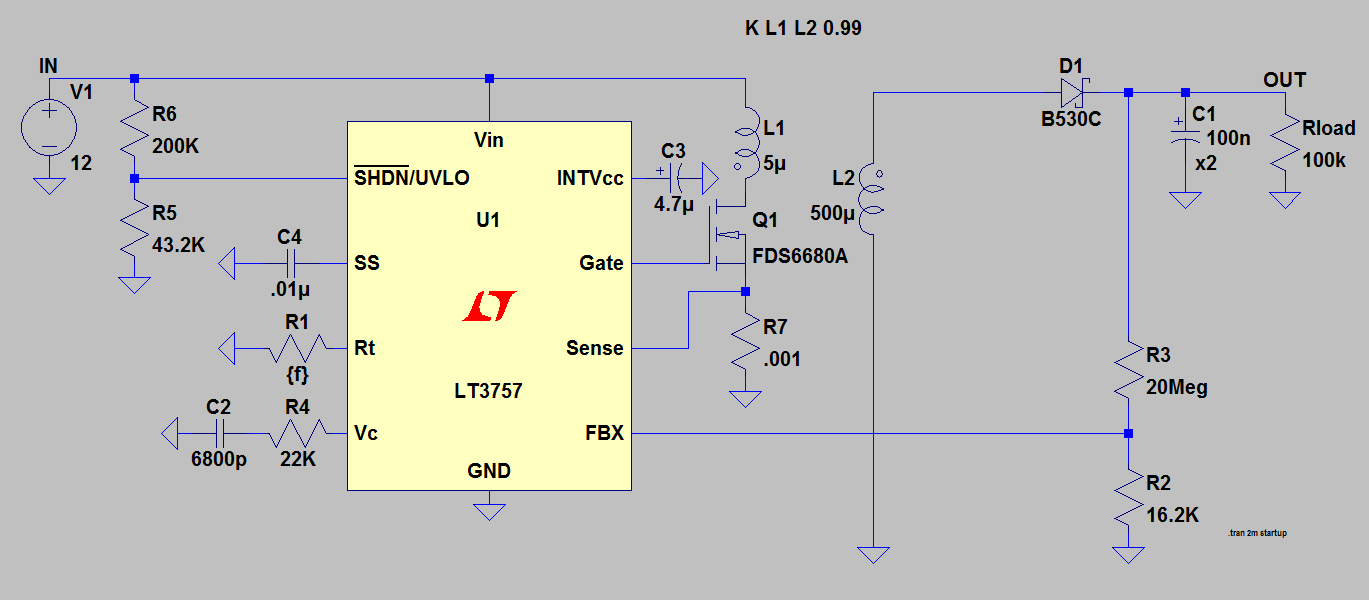
\includegraphics[width=1\columnwidth]{Slike/Simulacije/LM3757spice.png}
        \caption{\label{LM3757spice} Shema vezja v LTSpice.}
    \end{figure}
    
Problem tega krmilnika pa je varnost, ker je sekundarno navitje visokonapetostnega transformatorja električno povezano z nizkonapetostno stranjo. Za zagotavljanje primerne izolacije bi moral napajalnik modula zdržati \SI{15}{\kilo\volt}, kar ponovno pomeni načrtovanje takega napajalnika. Napajalniki z najvišjo prebojno trdnostjo so namreč s certifikatom IEC 60601-1, ki zagotavlja najvišjo prebojno trdnost \SI{4000}{\volt}AC.

	\subsubsection{LT8304} \label{LT8304}
LT8304 proizvajalca Linear Technology ~\cite{analog:LT8304} deluje po podobnem principu kot LM3748 z razliko, da ima vgrajen MOSFET in posledično manjšo izhodno moč. Simulacije so obetale, vendar jim ni moč zaupati zaradi netočnosti modela transformatorja. Vseeno sem poskusil izdelati prototipno ploščo s krmilnikom in pripadajočimi komponentami. Vezje je delovalo po pričakovanjih, vendar se je po približno 20 sekundah začelo kaditi iz krmilnika, zato sem uporabil nov krmilnik.
Tudi pri temu se je začelo kaditi. Ta krmilnik ima maksimalno moč \SI{24}{\watt}, pri meritvah pa moč ni presegla \SI{10}{\watt}. Dejstvo pa je, da je bil na izhodu napajalnika kondenzator s \SI{4700}{\micro\farad}, zaradi katerega napajalnik ni pokazal napetostnih špic, zaradi katerih je bila presežena izhodna moč. Drugi del, kjer bi lahko prišlo do napake je na pinu SW, ki je ponor internega MOSFETa. Mogoče je, da je inducirana napetost na primarnem navitju je višja od \(U_{DS MAX}\) in posledično poškoduje čip. Podatkovni list narekuje uporabo Schottky in Zenner diode s pragovno napetostjo \(V_{Zenner(MAX)} \leq 145 V - V_{IN(MAX)}\) proti napajalni liniji za odvajanje prenapetostnih špic. V mojem primeru sem uporabil Zenner diodo s pragovno napetostjo \SI{100}{\volt}, kar pa očitno ni zadoščalo. Na zadnjem krmilniku sem namesto priporočene prenapetostne zaščite uporabil TVS diodo, z nominalno napetostjo \SI{70}{\volt} in maksimalnim tokom \SI{26.5}{\ampere}. Vendar je bil rezultat še vedno isti.

    \subsubsection{Ugotovitve} \label{Ugotovitve glede komercialnih krmilnkov}
Simulacija so pokazale, da ne bo mogoče uporabiti že narejenega krmilnika, ampak ga bo potrebno načrtovati od začetka. Možna rešitev bi bila uporaba krmilnika LT3757, vendar bi bilo namesto napajanja z omrežnim napajalnikom potrebno uporabiti baterijsko napajanje. Baterije bi se polnile ob izklopu visokonapetostnega napajalnika, ob vklopu pa se baterije galvansko loči od polnilnika s pomočjo odklopnika,  ki ima prebojno napetost vsaj \SI{15}{\kilo\volt}. Takšen odklopnik pa ponovno pomeni veliko specifiko z visoko ceno oz. samoizdelavo. 

	\subsubsection{Krmilnik z mikrokrmilnikom} \label{KrmilnikzUc}
Edina možnost, ki nam je še preostala je bila izdelava visokonapetostnega krmilnika z mikrokrmilnikom. Krmilnik bo opravljal le vlogo krmiljenja visokonapetostnega napajalnika. Vhodni signal bo prejel preko serijske povezave, povratna vezava pa bo preko analogno-digitalnega pretvornika, ki bo na mikrokrmilnik povezan preko optičnega izolatorja za digitalne povezave. Uporabljen je bil mikrokrmilnik STM32 iz družine F4, ker njegove operacije niso tako kritične in lahko uporabimo kateri koli mikrokrmilnik. S STM Cube razvojim okoljem sem se že predhodno seznanil, razvojna ploščica STM NUCLEO F4 pa je bila na zalogi v podjetju. Analogno-digitalni pretvornik tudi ni bil kritičen, saj za koncept nismo potrebovali visoke natančnosti, galvansko ločitev med visokonapetostnim in nizkonapetostnim delom pa je zagotavljal digitalni izolator z vgrajenim izolatorjem napajanja iz družine ISOW proizvajalca Texas Instruments. 

	\begin{figure}[H]
    \centering
    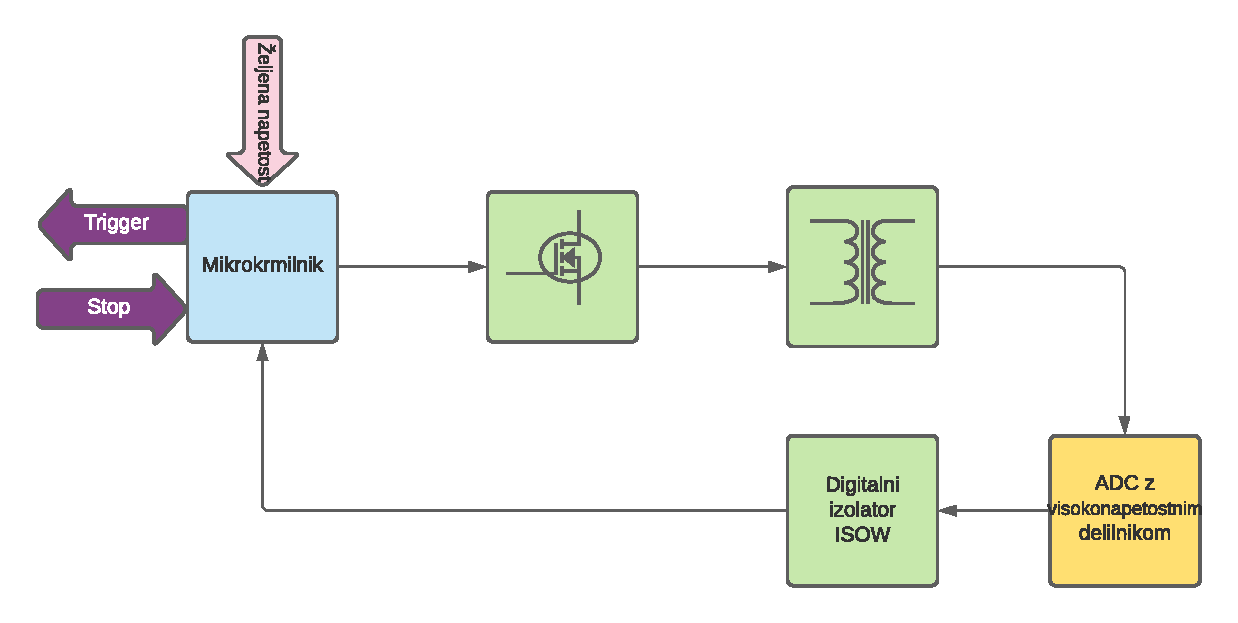
\includegraphics[width=1\columnwidth]{Sheme/KrmilnikzuCElShema.pdf}
    \caption{\label{KrmilnikzuCElShema} Shema visokonapetostnega krmilnika z mikrokrmilnikom.}
	\end{figure}

	\begin{figure}[H]
    \centering
    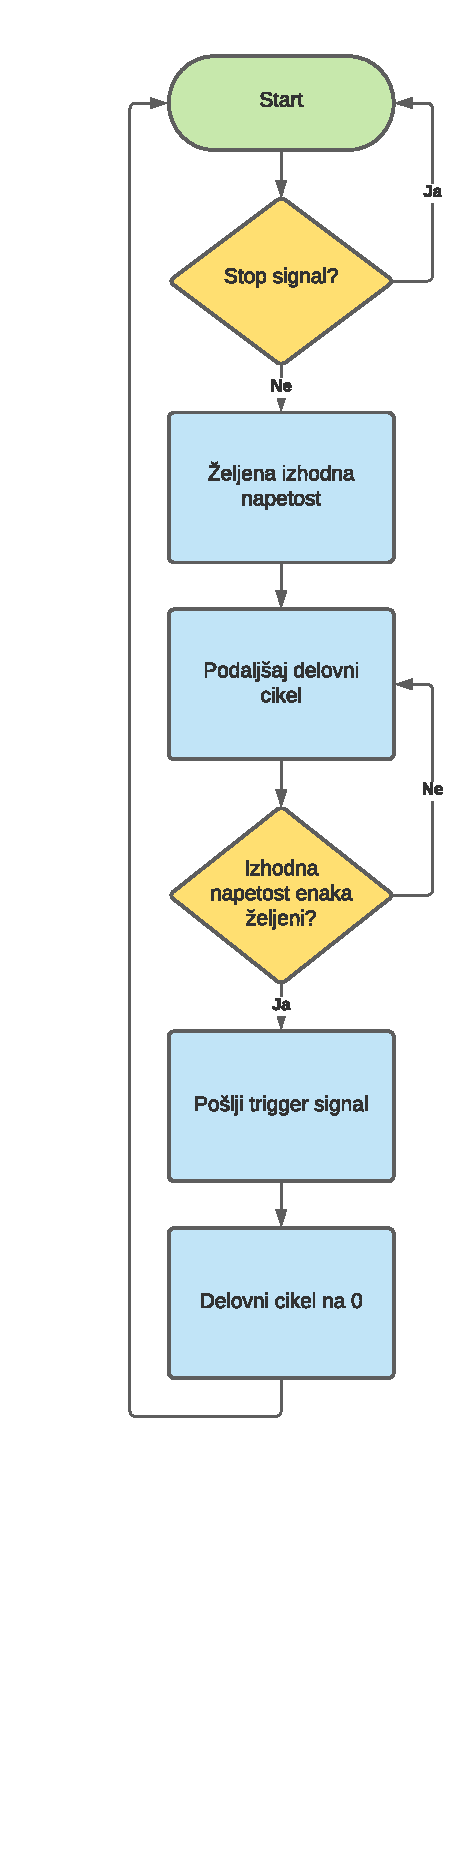
\includegraphics[width=0.35\columnwidth]{Sheme/KrmilnikzuCShema.pdf}
    \caption{\label{KrmilnikzuCShema} Shema programske kode visokonapetostnega krmilnika z mikrokrmilnikom.}
	\end{figure}
	
Programska koda preveri, če glavni krmilnik še pošilja STOP signa. 

Če ga ne pošilja, prebere željeno napetost preko serijske povezave in nastavi delovni cikel na najkrajšega. Dokler izhodna napetost ne doseže nastavljene, počasi povečuje delovni cikel. Ko izhodna napetost doseže nastavljeno, pošlje glavnemu krmilniku TRIGGER signal, to je signal, ki sproži praznilni rele in postavi delovni cikel na 0. Počasno dviganje napetosti omogoča počasnejše polnenje kondenzatorja in posledično je potreben manjši transformator. S tem krmilnikom je uspelo krmiliti izhodno napetost, potrebno pa bi bilo še podrobneje nastaviti PID parametre.

	\subsection{Visokonapetostno stikalo} \label{Visokonapetostno stikalo}
	Standard zahteva ''bounce-less'' stikalo stikalo, ki sklene kontakt in ga ne razklene več. V preteklosti so bili na voljo, ki so imeli kontakte v kapsuli skupaj z živim srebrom. Živo srebro je poskrbelo, da v času ko sta bila kontakta odbita je tok lahko še vedno tekel preko živega srebra. Vendar je zaradi direktive RoHS izbira teh relejev zelo omejena.
	
	\subsubsection{Komercialno dobavljivi releji} \label{Komercialno dobavljivi releji}
     Prvotna izbira je bil model G61A proizvajalca Gigavac ~\cite{Gigavac:G61A}, ki se vgrajuje v simulatorje elektrostatične razelektritve, saj je v specifikacijah poudarjeno ''Odličen za praznjenje kondenzatorjev ter efektivno operira brez skakanja kontaktov.''
    
    \begin{figure}[H]
        \centering
        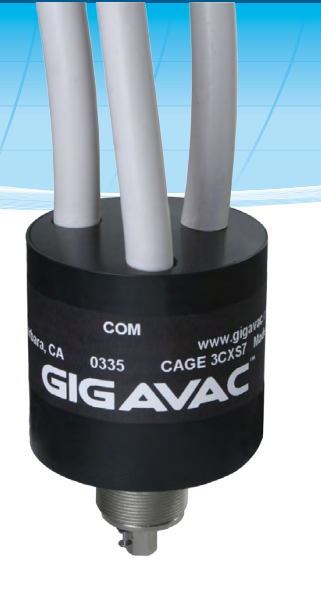
\includegraphics[width=0.5\columnwidth]{Slike/GigavacG61C.png}
        \caption{\label{GigavacG61C} Slika releja G61A proizvajalca Gigavac.}
    \end{figure}    
    
    Cena tega releja giba okoli 2000\euro{}. Zaradi omejenega proračuna nakup tega releja ni bil možen. Dobro alternativo je predstavljal rele serije H, proizvajalca Medler electronics ~\cite{Standex:H} (sedaj Standex electronics), ki ima v specifikacijah navedeno ''Zamenjava za mokre releje z živim srebrom'' in je bil na voljo po ugodni ceni 50\euro{}.
    
Testi so po pričakovanju pokazali skakanje kontaktov.
    
    \begin{figure}[h]
        \centering
        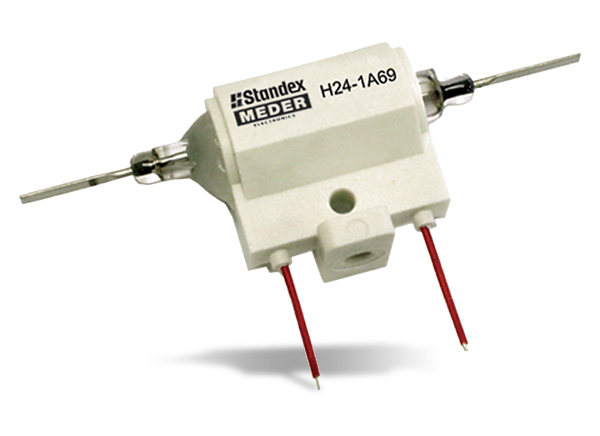
\includegraphics[width=1\columnwidth]{Slike/MederReleH.png}
        \caption{\label{MederReleH} Slika releja serije H proizvajalca Meder.}
    \end{figure}        
    
    \begin{figure}[H]
    \centering
        \begin{circuitikz}
           \draw (2,1)
            to[V, v=$Sig$] (2,3)
            to[short] (4,3)
            to[L] (4,1)
            to[short] (2,1);
        
           \draw (0,0)
            to[short] (0,1)
            to[C=10 nF] (0,3)
            to[short] (0,4)
            to[R=10 Ohm] (5,4)
            to[normal open switch] (5,0)
            to[short] (0,0);
    
        \draw (2.5,6) node[oscopeshape](osc1){}
        (osc1.left) node[anchor=west] {}
        (osc1.right) node[anchor=east] {};
        
        \draw (osc1.left)
        to[short] (0,6)
        to[short] (0,4);
        
        \draw (osc1.right)
        to[short] (5,6)
        to[short] (5,4);
        
        \draw (0,4) node[circ]{};
        \draw (5,4) node[circ]{};
	\end{circuitikz}
	   \caption{\label{MerilnoVezjeRele} Shema vezja za merjenje relejev.}
    \end{figure}
    
    \begin{figure}[H]
        \centering
        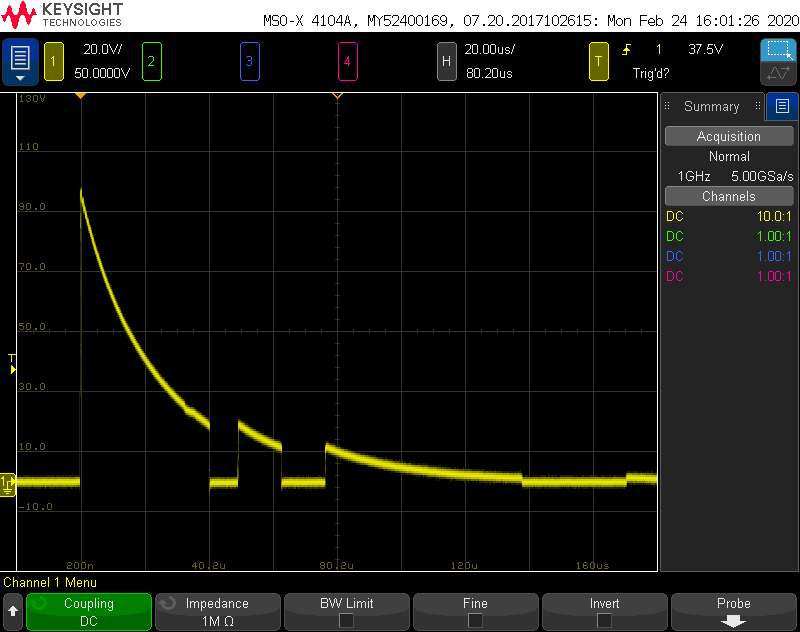
\includegraphics[width=1\columnwidth]{Slike/MedlerElectronicsRele.png}
        \caption{\label{BlokDiagramShema} Skakanje kontaktov pri releju proizvajalca Medler electronics.}
    \end{figure}
    
    ~\\Po specifikacijah je lahko največji tok, ki teče čez rele \SI{10}{\ampere}, saj je maksimalna napetost \SI{15}{\kilo\volt}, kondenzator pa se prazni preko \SI{1500}{\ohm} upora. Zaradi varnosti je bila pri merjenju RC konstanta spremenjena iz \SI{1500}{\ohm} in \SI{100}{\pico\farad} na \SI{10}{\ohm} in \SI{10}{\nano\farad}, napajana pa je bila z napetostjo \SI{100}{\volt}. Na posnetku zaslona osciloskopa je razvidna razklenitev pri \SI{40}{\micro\second} in \SI{55}{\micro\second}. Po ponovitvah sem zaključil, da so razklenitve pojavijo vedno ob istem času. Pojavila se je ideja o vzporednem vezanju dveh ali več enakih relejov in njihovem porženju s časovnim zamikom, ker bi na ta način lahko premostili razklenitev. Vendar bi s tem v sistem dodali kapacitivnost na katero moramo biti zelo pozorni, saj standard dovoljuje maksimalno \SI{20}{\nano\second} odstopanja časovne konstante.
Eksperimentalno sem naredil meritve še pri višjih napajalnih napetostih vzbujevalne tuljave, kjer sem predpostavljal, da bo magnetno polje dovolj močno, da se kontakt ne bo uspel odbiti. Kljub temu so se prekinitve še vedno dogajale, tudi pri trojni napajalni napetosti.
   
	\subsubsection{Komercialna tranzistorska rešitev} \label{Komercialna tranzistorska rešitev}   
    
	Podjetje Behlke, ki se ukvarja z visokonapetostno in močnostno elektroniko, izdeluje HTS 181-02-C ~\cite{Behlke:HTS181-02-C} hitro visokonapetostno tranzistorsko stikalo. Ta model ima maksimalno napetost \SI{18}{\kilo\volt} ter maksimalno tokovno špico \SI{12}{\ampere}. Nekoliko slabši so parametri časa naraščanja, saj bi bili v našem primeru med \SI{12}{\nano\second} do \SI{25}{\nano\second} (standard pa zahteva \SI{10}{\nano\second}). Tako stikalo ima ceno okoli 1100\euro , kar je močno presegalo naš proračun. Po ogledu fotografije odprtega stikala sem si zamisli, kako bi potekala lastna izvedba tranzistorskega visokonapetostnega stikala.
	
	\subsubsection{Samogradnja tranzistorskega visokonapetostnega stikala} \label{Samogradnja tranzistorskega visokonapetostnega stikala}
	
	Stikalo je sestavljeno iz dveh delov: krmilni del in visokonapetostni del. Zanimivo je dejstvo, da je v visokonapetostnem delu zaporedno nanizanih okoli 10 tranzistorjev. Če predpostavimo, da imajo vsi tranzistorji enake karakteristike in se v istem času začnejo odpirati, bo napetost naraščala na vseh enako in skupni dvižni čas bo enak dvižnemu času tranzistorja. Prva izziv se je pojavil glede izbire primernih polprevodnikov. IGBTji IXYL60N450 ~\cite{IXYS:IXYL60N450} proizvajalca LittleFuse so bili teoretično najboljša izbira, saj imajo maksimalno \(V_{CES}\) napetost \SI{4.5}{\kilo\volt}, tipični odpiralni čas pa je \SI{55}{\nano\second}, kar je še vedno 5.5 krat preveč. 

    Naknadno sem naletel na tranzistorje, ki so bili namenjeni za \SI{10}{\kilo\volt} z dvižnim časom okoli \SI{10}{\nano\second}. Mogoče bi bilo uporabiti dva in ju zbondirali na tiskano vezje in s tem zmanjšali parazitne kapacitivnosti in induktivnosti. Zaradi hitrega dvižnega časa spadajo ti tranzistorji pod ''izdelke z dvojnim namenom'', kar pomeni, da je za nakup potrebno podpisati pogodbo o nerazkritju informacij. Najnižje vrednosti parazitne kapacitivnosti in induktivnosti bi tako lahko dosegli z uporabo najbolj primernih tranzistorjev odstranjenih iz ohišja in zbondiranih na tiskano vezje. Pred risanjem tiskanega vezja sem želel v simulatorji zasnovati še krmilnik. Uporabljeni so bili IGBTji, zato je bilo potrebno krmilno napetost pripeljati med vrata in emitor. V mojem primeru je potencial emitorja najvišjega IGBTja proti masi znašal \SI{11.25}{\kilo\volt}. S primernimi visokonapetostnimi stikali bi bilo možno krmiljenje na način s preklopi kondenzatorja t.i. ''Switched Cap''.

    %shema swtiched cap
    \begin{figure}[H]
    \centering
        \begin{circuitikz}
            \draw (0,0)
            to[V, v=$Sig$] (0,3)
            to [short] (1.185,3)
            to[short] (1.185,2.85);
            
            \draw (1.5,2.3)
            node[spdt, rotate=90] (sw1) {}
            (sw1.in) node[left] {};
            
            \draw (1.5,0.7)
            node[spdt, rotate=-90, yscale=-1] (sw2) {}
            (sw2.in) node[left] {};;
             
            \draw (sw1.in)
            to[C] (sw2.in);
           
            \draw  (1.815,0.15)
            to[short] (1.815,0)
            to[short] (4,0)
            to[short] (4,1.5);
            
            \draw (4,2)
		node[nigfetd](Q){}
		(Q.G) node[left] {};
		
		
		
		
		
		
		
		\draw (Q.G) to[short] (3.0145,3)
		to[short] (1.815,3)
		to[short] (1.815, 2.85);
		
		\draw (0,0)
            to[short] (1.185, 0)
            to[short] (1.185, 0.15);    
        \end{circuitikz}
                \caption{\label{SwitchedCapFetDriver} Shema idejne zasnove krmiljenja tranzistorja preko ''Switched Cap''.}
    \end{figure}
    V članku avtorjev Continetti, R. E., Cyr, D. R., and Neumark, D. M\cite{doi:10.1063/1.1143294} so opisali podoben problem, ki so ga reˇsevali s transformatorji v razmerju 1:1 in primerno prebojno trdnostjo. V simulacijah se je rešitev obnesla. V resničnem svetu pa se to verjetno ne bi obneslo, saj bi le majhna zakasnitev posameznega krmilnika ali tranzistorja povzročila, da bi na njem pristala celotna napetost in posledično seveda preobremenitev.
    
	\subsubsection{Mehanska rešitev} \label{Mehanska rešitev}    
    
    
    V iskanju nadaljnjih rešitev je bil logičen zaključek mehanska rešitev z enim stikalom, brez zaporedne ali vzporedne vezave stikal. V nadaljevanju so predstavljeni prototipi štirih stikal:
    \begin{enumerate}
   
        \item  Solenoid drži razklenjena kontakta, ki ju skupaj ju vleče vzmet. Ob sprožitvi se obrne polariteta napajanja tuljave solenoida, ki poleg vzmeti vleče kontakta skupaj.
    \begin{figure}[H]
        \centering
        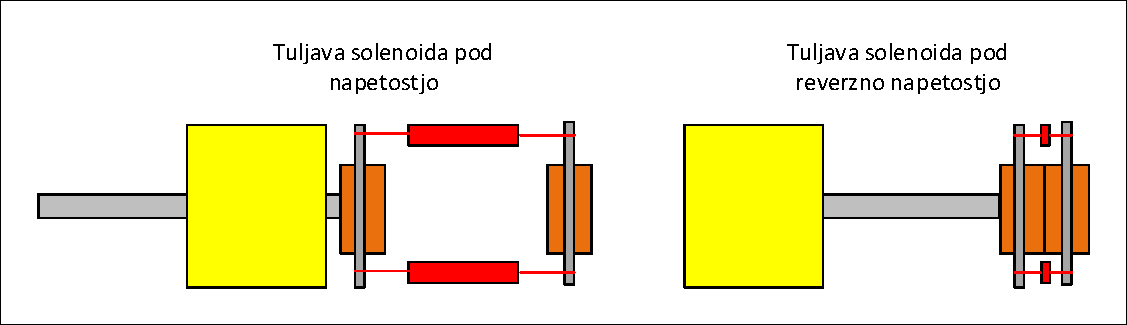
\includegraphics[width=1\columnwidth]{Sheme/StikaloSolenoidVerzija1.pdf}
        \caption{\label{/StikaloSolenoidVerzija1} Shema stikala s solenoidom V1.}
    \end{figure}
    
    \item  Solenoid, ki porine kontakt, jezička pa ga ujameta.
    \begin{figure}[H]
        \centering
        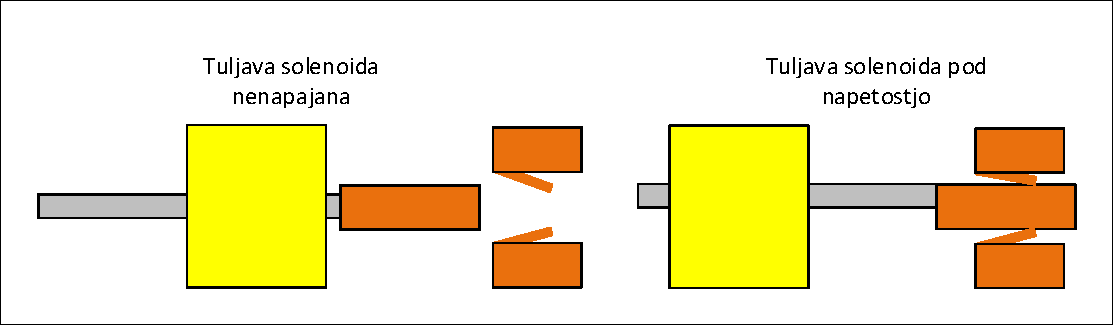
\includegraphics[width=1\columnwidth]{Sheme/StikaloSolenoidVerzija2.pdf}
        \caption{\label{/StikaloSolenoidVerzija2} Shema stikala s solenoidom V2.}
    \end{figure}
    
    \item  Servo motor se zasuče in z drsnim stikalom sklene kontakt.
    \begin{figure}[H]
        \centering
        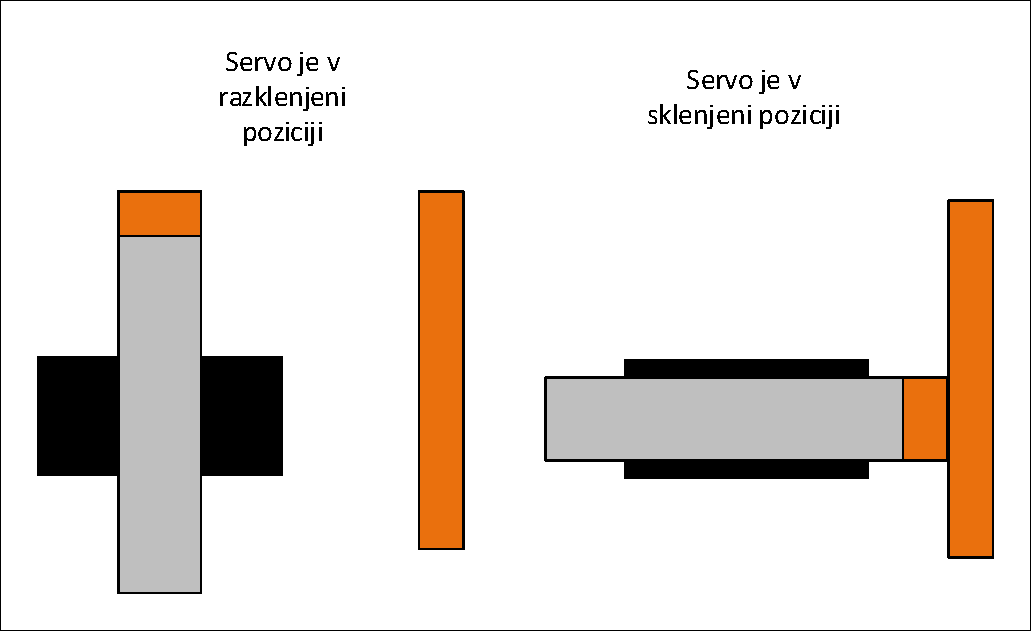
\includegraphics[width=1\columnwidth]{Sheme/StikaloServoVerzija1.pdf}
        \caption{\label{StikaloServoVerzija1} Shema stikala s servo motorjem V1.}
    \end{figure}
    
    \item  Servo motor se zasuče in pritisne na kontakt kateri je na vzmeti.
    \begin{figure}[H]
        \centering
        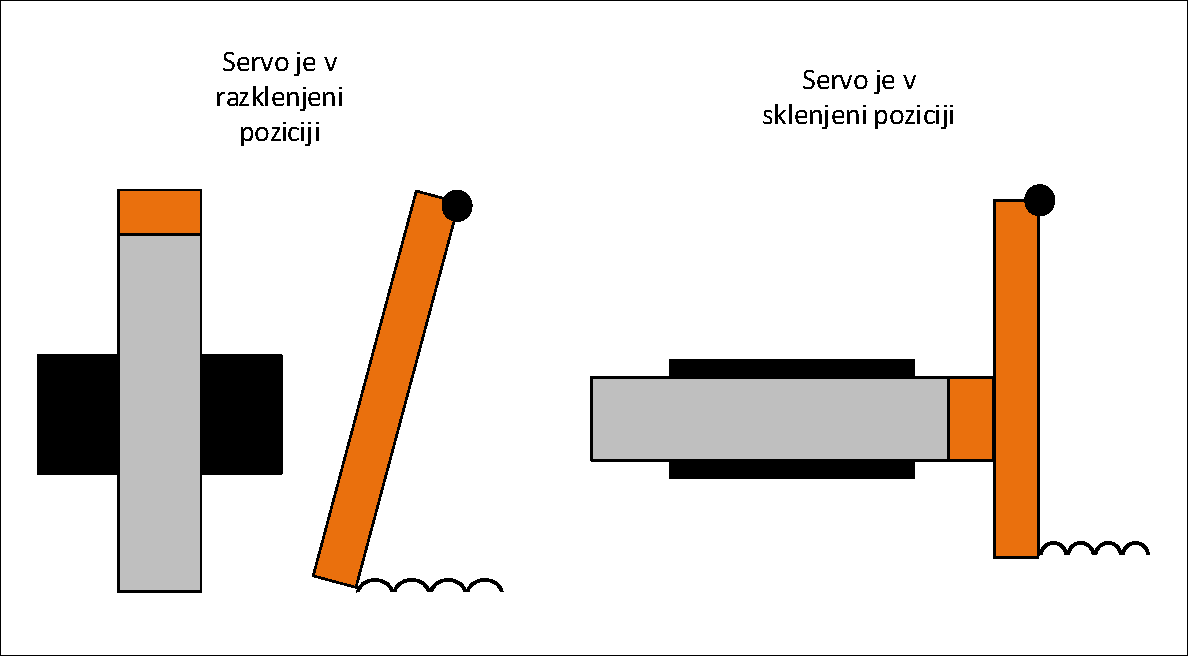
\includegraphics[width=1\columnwidth]{Sheme/StikaloServoVerzija2.pdf}
        \caption{\label{StikaloServoVerzija2} Shema stikala s servo motorjem V2.}
    \end{figure}
\end{enumerate}


    ~\\Za solenoid je bil najprej uporabljen manjši model, ki je bil namenjen konstantnemu delovanju pri \SI{12}{\volt}, za hitrejˇse delovanje in veˇcjo silo pa se ga lahko prenapaja s \SI{40}{\volt} za čas  \SI{1}{\second} z delovnim ciklom 5\%. Ta model se je izkazal za neprimernega, saj v trenutku, ko se je na njega namestil kontakt, ni imel več zadostne moči za premikanje, še posebno, če bi se moral upirati sili vzmeti. 
~\\ 
~\\Za hitri preizkus postavljene teze sem sestavil solenoid na tuljavniku transformatorja.
    %probat še z močnejšim solenoidom
    
    ~\\Za hitri preizkus postavljene teze sem sestavil solenoid na tuljavniku
transformatorja. 
~\\Meritve prototipa stikala V1 s servo motorjem so pokazale dvižni čas \SI{10}{\nano\second}, vseeno pa so se pojavljale manjše prekinitve po sklenitvi kontaktov. Poleg tega bi lahko problem predstavljala tudi obraba in oksidacija kontaktov. Rešitev bi bila zaprtje celotnega stikala v vakuumsko komoro ali še bolje v plin $SF_{6}$ kateri ima zelo visoko prebojno trdnost.
    
    \begin{figure}[H]
        \centering
        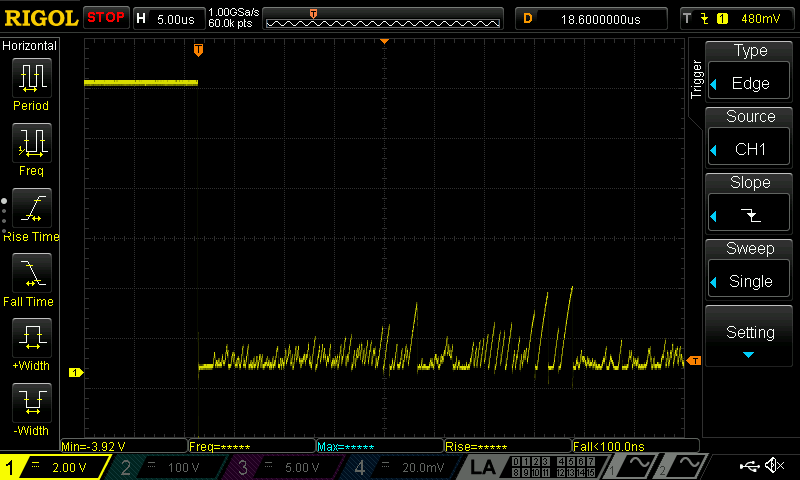
\includegraphics[width=1\columnwidth]{Slike/ServoStikalo1/ServoStikalo1.png}
        \caption{\label{ServoStikalo1} Potek napetosti po sklenitvi kontaktov pri servo stikalu V1.}
    \end{figure}
    
    \begin{figure}[H]
        \centering
        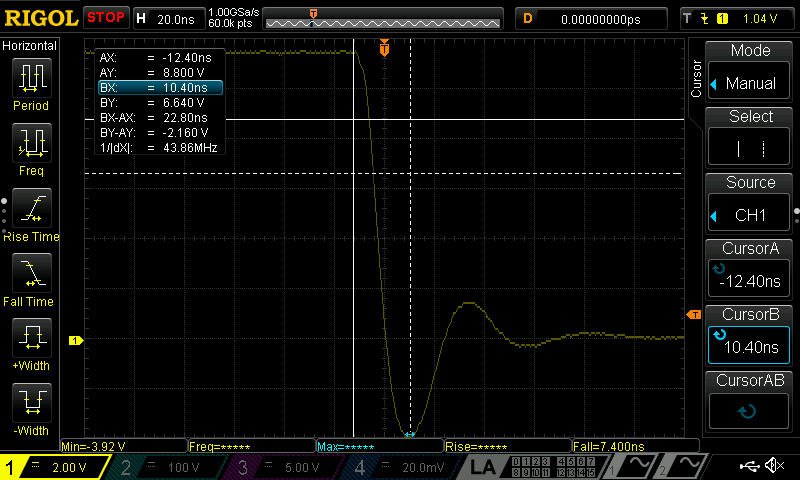
\includegraphics[width=1\columnwidth]{Slike/ServoStikalo1/ServoStikalo1povecano.png}
        \caption{\label{ServoStikalo1povecano} Potek napetosti po sklenitvi kontaktov pri servo stikalu V1 povečano.}
    \end{figure}
    
    ~\\Pri stikalu V2 s servo motorjem pa se je pojavil izziv počasnega dvižnega časa. Predvidoma jo povzroča vsa parazitna kapacitivnost. Potrebno bi bilo narediti revizijo in skrajšati vse segmente žice ter izdelati bolj kompaktne kontakte.
    





\chapter{Sklep} \label{Sklep}

Sama zasnova projekta je bila izredno smelo zastavljena, kar se tiče časovnih okvirjev in proračuna, ob sami izvedbi pa nismo pričakovali takih zapletov.
~\\Veˇcji del izziva je predstavljala zahtevana visoka napetost, saj so komercialno
dosegljive komponente dobavljive do \SI{3}{\kilo\volt}, za višje napetosti pa postanejo komponente težje dobavljive in posledično dražje. Veliko preglavic je povzročal tudi rele brez skakanja, saj se načeloma uporablja za nizke napetosti. Poleg tega vsebuje nevarne substance, kar ga naredi še težje dostopnega. Kljub temu sem z eksperimenti prišel do nekaj uporabnih rešitev, ki jih bom bolje raziskal pri izdelavi diplomske naloge. Kot ESD simulator bi lahko uporabil komercialni visokonapetostni nastavljivi napajalnik proizvajalca Applied Kilovolts in visokonapetostni rele, namenjen praznjenju kapacitivnih zalogovnikov
proizvajalca Gigavac, vendar bi taka rešitev podražila projekt za približno 5000\texteuro . Druga možnost je bila lastni razvoj visokonapetostnega nastavljivega
napajalnika in visokonapetostnega releja, ki bi podobno podražila projekt, vendar bi zahtevala dodatno 400 ur dela. Dodatno pa tudi podjetje nima izkušenj s tako visokimi napetostmi, saj se ukvarja z mikroelektroniko.


\bibliographystyle{acm}	
\bibliography{literatura} 




\end{document}
%%%%%%%%%%%%%%%%%%%%%%%%%%%%%%%%%%%%%%%%%%%%%%%%%%%%%%%%%%%%%%%%%%%%%%%%%%%%%%%%%%%%%%%%%%%%%%%%%%%%%%%%%%%%%%%%%%%%%%%%
